\documentclass[11pt]{article}
% Use the official ACL style when compiling in the ACL Overleaf project.
% The fallback below only enables an offline PDF preview; it is NOT the ACL style.
\IfFileExists{acl.sty}{\usepackage{acl}}{\usepackage[margin=0.84in,columnsep=0.27in]{geometry}\usepackage{natbib}\twocolumn}
\usepackage[T1]{fontenc}
\usepackage[utf8]{inputenc}
\usepackage{times}
\usepackage{latexsym}
\usepackage{graphicx}
\setkeys{Gin}{draft=false} % Render figures even if a draft option is inherited
\usepackage{booktabs}
\usepackage{array}
\usepackage{multirow}
\usepackage{url}
\usepackage{amsmath}
\usepackage{microtype}
\usepackage{xcolor}
\usepackage{float}
\usepackage{caption}
\newcommand{\ap}{\mathrm{AP}}
\newcommand{\roc}{\mathrm{ROC\mbox{-}AUC}}
\newcommand{\repository}{\textbf{[ADD PUBLIC GITHUB URL BEFORE SUBMISSION]}}
\emergencystretch=2em
\sloppy
\title{Reproducing and Extending OptIForest for Anomaly Detection: Replication, Controlled Ablations and Synthetic Transaction Experiments}
\author{Zeki Kose\\48718459\\Macquarie University, COMP8240\\\texttt{zeki.kose@students.mq.edu.au}}
\date{}
% Ensure hyperref is loaded exactly once (ACL may load it internally).
\makeatletter
\@ifpackageloaded{hyperref}{}{\usepackage{hyperref}}
\makeatother
\hypersetup{
    colorlinks=true,
    linkcolor=blue,
    citecolor=blue,
    urlcolor=blue
}

\begin{document}
\maketitle
\begin{abstract}
This default-project study examines the reproducibility and limited generalisation of OptIForest, an isolation-based unsupervised anomaly detector with learned hierarchical partitions. We executed the public implementation on its supplied AD benchmark, constructed an Isolation Forest baseline, and investigated branching and cut-threshold choices. We also generated nine reproducible synthetic transaction datasets covering point, contextual and collective anomalies at 1\%, 5\% and 10\% prevalence. Our original-data replication achieved mean ROC-AUC 0.7741 and average precision (AP) 0.4351, closely matching published figures of 0.774 and 0.438. In three-seed branching experiments, fixed ternary branching gave higher mean AP (0.4498) than the expected-$e$ mixed setting (0.4264), although the small number of repeats limits inference. On synthetic data, same-seed comparisons favour OptIForest for point anomalies but generally favour standard Isolation Forest for contextual and collective anomalies. Results expose meaningful dependence on anomaly mechanism, parameter settings and substantial scoring costs. We explicitly distinguish single-seed observations from repeated-run conclusions and describe the reproducibility and ethical limitations of the work.
\end{abstract}
 
\section{Introduction and Research Basis}
Anomaly detection identifies observations that differ from expected patterns. Applications include network monitoring, financial transaction screening and industrial fault detection. Rare anomalies, heterogeneous mechanisms and limited labels complicate evaluation \citep{pang2021}. Isolation Forest (iForest) addresses the problem without supervised labels by exploiting the tendency of unusual observations to be isolated after fewer random partitions \citep{liu2008,liu2012}.
 
OptIForest, proposed by \citet{xiang2023} at IJCAI 2023, extends the isolation-tree family through a multi-fork construction and a clustering-oriented learning-to-hash mechanism. Its authors argue for an expected branching factor near Euler's number $e$, implemented by probabilistically combining binary and ternary merges. The paper evaluates multiple benchmarks and reports ROC-AUC, precision--recall performance and parameter studies. The official code and its supplied \texttt{ad.csv} dataset are available online.\footnote{Original OptIForest project: \url{https://github.com/xiagll/OptIForest}.}
 
This project follows the individually proposed \emph{default project}. Its questions are: \textbf{RQ1}: Can reported OptIForest performance on the supplied AD benchmark be reproduced? \textbf{RQ2}: How do branching choice and cut threshold affect performance and runtime? \textbf{RQ3}: Does OptIForest outperform a transparent iForest baseline for different synthetic anomaly mechanisms and prevalence levels? Proposed hypotheses included numerical reproduction within five percentage points (H1), mixed branching within 0.02 AP of the best fixed branch (H2), and positive paired AP differences on new datasets (H3). We report observations even where they contradict expectations.
 
\section{Original Dataset and Replication}
\subsection{Data and reproducible environment}
The public repository supplies one original dataset, \texttt{data/ad.csv}, containing 3,279 records with 1,555 numeric features and a final binary label. There are 2,820 normal and 459 anomalous observations, with no missing values reported in the proposal's data inspection. This is a supplied benchmark, not a real banking dataset. The 20 datasets studied in the original paper are not all bundled with the accessible code; therefore, this project does not claim to reproduce the entire published benchmark suite.
 
The local experiments used Python 3.12 and current NumPy, SciPy, pandas and scikit-learn libraries on Windows. An initial compatibility failure occurred because modern NumPy removed \texttt{np.mat}. Two affected calls were replaced by \texttt{np.asmatrix} without an intended change to the algorithm. Both the original-code source and the small compatibility changes should be documented in the companion repository. The work also repeatedly emitted a runtime warning for an invalid scalar division within the tree implementation; since the affected numerical path was not formally audited, this warning is a reproducibility limitation rather than proof of correct numerical behaviour.
 
\subsection{Experimental protocol}
The original-data replication uses the provided \texttt{L2OPT} variant, 100 trees, sample size 512, cut threshold 403 and branch setting 0 (probabilistic mixed branching). The full unlabeled feature matrix is used for unsupervised fitting and scoring, consistent with the repository's transductive protocol; labels are withheld from fitting and used only for evaluation. Original AD features are \emph{not} scaled. The original demo records 15 stochastic repetitions. A local scikit-learn \texttt{IsolationForest} baseline uses 100 estimators, a maximum subsample of 512, seed values 0--14 and the negative of its native score as anomaly evidence.
 
We calculate ROC-AUC and scikit-learn \texttt{average\_precision\_score}. The repository labels the latter metric AUC-PR; this report calls it \emph{average precision} (AP) because AP and trapezoidal PR-AUC are related but not mathematically identical. Timing records separate model fitting and scoring. A transductive protocol facilitates code-faithful comparison but does not evaluate generalisation to unseen future transactions.
 
\subsection{Replication results}
\begin{table}[t]
\centering\small
\caption{Original AD benchmark: reported OptIForest values and local replication. Values are means $\pm$ reported SD across 15 runs (original demo uses population SD; iForest summary uses sample SD).}
\label{tab:replication}
\begin{tabular}{@{}lcc@{}}
\toprule
System & ROC-AUC & AP / reported PR \\
\midrule
Paper OptIForest & $0.774\pm0.007$ & $0.438\pm0.031$ \\
Local OptIForest & $0.7741\pm0.0057$ & $0.4351\pm0.0294$ \\
Local iForest & $0.6878\pm0.0213$ & $0.3929\pm0.0531$ \\
\bottomrule
\end{tabular}
\end{table}
 
Table~\ref{tab:replication} demonstrates close numerical agreement with the published AD row: the replicated means differ from the paper by roughly 0.0001 ROC-AUC and $-0.0029$ AP. This supports H1 for the accessible original experiment. The original demo's aggregated output reported mean OptIForest fitting and scoring times of 24.34 and 55.50 seconds, respectively; corresponding local iForest means were 0.136 and 0.024 seconds. The 15 individual OptIForest AD rows were not included in the latest archived results ZIP; the reported mean and standard deviation derive from the preserved original demo output. They should not be misrepresented as a presently archived raw 15-row CSV.
 
\section{Branching and Threshold Ablations}
Ablations used the original AD dataset without scaling, 100 trees, the same feature matrix and evaluation definitions. Branch choices 0 (mixed), 2 (fixed binary) and 3 (fixed ternary) were compared at threshold 403 with matched model seeds 0, 1 and 2. Figure~\ref{fig:branch} and Table~\ref{tab:branches} present sample means and standard deviations. These are modest repeated experiments, not a full statistical reproduction of the paper's ablation suite.
 
\begin{table}[t]
\centering\small
\caption{Three-seed AD branching study (threshold 403). Values are mean $\pm$ sample SD.}
\label{tab:branches}
\begin{tabular}{@{}lcc@{}}
\toprule
Branch & ROC-AUC & AP \\
\midrule
Mixed (0) & $0.7713\pm0.0029$ & $0.4264\pm0.0098$ \\
Binary (2) & $0.7659\pm0.0038$ & $0.3845\pm0.0039$ \\
Ternary (3) & $0.7752\pm0.0048$ & $0.4498\pm0.0322$ \\
\bottomrule
\end{tabular}
\end{table}
\begin{figure}[t]
\centering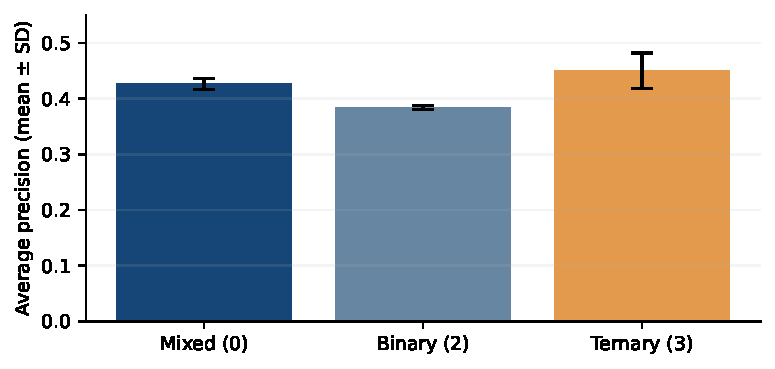
\includegraphics[draft=false,width=.94\columnwidth]{figures/branch.pdf}
\caption{Branch mean AP with sample standard-deviation bars across seeds 0--2.}
\label{fig:branch}
\end{figure}
 
The fixed ternary configuration achieved the highest three-seed mean AP (0.4498), ahead of mixed branching (0.4264) and binary branching (0.3845). Ternary branching also had the highest variability ($s=0.0322$). The mean AP deficit of mixed relative to ternary is about 0.0234, slightly greater than the proposed H2 tolerance of 0.02. Thus, H2 is \emph{not supported by these three seeds}; three runs are too few to conclude reliable superiority of ternary branching. The seed-0 outcome alone had favoured mixed branching, underscoring why repetitions matter.
 
\begin{table}[t]
\centering\small
\caption{Single-seed AD threshold ablation with branch 0. Total time is fitting plus scoring. Threshold 7 did not complete.}
\label{tab:threshold}
\begin{tabular}{@{}rrrr@{}}
\toprule
Threshold & ROC-AUC & AP & Time (s) \\
\midrule
20 & 0.7563 & 0.3664 & 3515.8 \\
55 & 0.7660 & 0.3919 & 267.4 \\
148 & 0.7613 & 0.3711 & 101.4 \\
403 & 0.7722 & 0.4256 & 81.6 \\
512 & \textbf{0.7836} & \textbf{0.4611} & \textbf{37.5} \\
\bottomrule
\end{tabular}
\end{table}
 
Thresholds 20, 55, 148, 403 and 512 were each evaluated with seed 0. Threshold 7 was attempted twice but interrupted during tree construction; neither attempt produced a completed metric, and none is invented here. Within the five completed settings, threshold 512 attained the highest AP (0.4611) and the shortest total recorded time (37.5 seconds). Threshold 20 took about 58.6 minutes, dominated by fitting, compared with 37.5 seconds at 512. The trend is not monotonic in AP (55 exceeded 148), and single-seed ablations do not establish a globally optimal threshold. The rapidly increasing computation at low thresholds is an important practical constraint on a complete grid search.
 
\section{Synthetic Transaction Data}
\subsection{Generation and provenance}
Nine controlled CSV datasets were generated with a seeded Python script and 10,000 transactions each: three anomaly mechanisms crossed with prevalence levels of 1\%, 5\% and 10\%. In each dataset, the number of positive labels is respectively 100, 500 or 1,000; the remaining records are normal. The eight numeric features are transaction amount, hour, account age in days, distance from usual location, number of transactions in 24 hours, merchant risk, device familiarity, and geographic velocity. No genuine customer information or personal identifiers were collected.
 
The generator creates a mixture of three normal customer profiles with different amount, activity and geographical patterns. It then selects anomaly indices using a deterministic \texttt{numpy.random.default\_rng(seed)} stream. \emph{Point anomalies} receive extreme amounts and geographic velocities. \emph{Contextual anomalies} receive individually plausible but unusual combinations of early-hour transactions, large distances and low device familiarity. \emph{Collective anomalies} simulate high-frequency bursts with elevated velocities and characteristic times and amounts. Importantly, collective cases are simulated as a collection of similarly distributed burst records, \emph{without stored customer identifiers or explicit event links}; the experiment therefore cannot verify relational group detection or temporal sequence reasoning.
 
Each CSV has a JSON sidecar recording the generator seed, anomaly mechanism, requested and realised prevalence, feature list, label distribution and SHA-256 checksum. The three initial 5\% datasets passed automated validation. For final packaging, all nine CSV files were regenerated or checked with the stored script and then passed the validator for row counts, class prevalence, missing values, deterministic reproduction and checksum integrity. This verifies internal consistency, not behavioural realism.
 
\begin{table}[t]
\centering\small
\caption{Example schema and dataset composition. Feature values are generated, not real transactions.}
\label{tab:data}
\begin{tabular}{@{}ll@{}}
\toprule
Column example & Meaning \\
\midrule
\texttt{amount} & Synthetic transaction value \\
\texttt{hour} & Time of day, 0--23 \\
\texttt{transactions\_24h} & Recent activity count \\
\texttt{device\_familiarity} & Simulated device familiarity \\
\texttt{label} & 0 normal, 1 injected anomaly \\
\midrule
Rows per dataset & 10,000 \\
Anomalies at 1\% / 5\% / 10\% & 100 / 500 / 1,000 \\
\bottomrule
\end{tabular}
\end{table}
 
 
\subsection{Checks on the generated data}
The validity of these datasets is more than obtaining the intended class count. For each new configuration, deterministic generation means that the same script version and seed can reproduce the same CSV bytes. The hash in the JSON metadata is useful for confirming identity of an archived file; it does not independently prove that the design represents realistic financial behaviour. The initial validation routine also checks feature domains, absent values, prevalence and repeatability, but it cannot establish ecological validity or effective isolation of anomaly mechanisms. Because the data-generating intervention directly modifies the model features, an apparently impressive detection score may partly reflect deliberately separable synthetic signals.
 
The normal customer profiles are mixture components with differing spend levels, hour distributions and activity rates. Thus a row that is unusual relative to a global distribution might nevertheless be normal for its customer profile, which motivates contextual testing. Yet the generator does not retain a customer-profile identifier in the delivered feature matrix. The data therefore test anomaly ranking under controlled distributions rather than genuine personalised context. Collective anomalies present a stronger mismatch: records are modified together in terms of frequency and hour ranges, but the dataset contains no persistent account ID, linked transaction graph or sequential event index. It is not possible to evaluate whether either model recognises a coordinated group as a group; the experiments instead test whether unusual individual feature combinations corresponding to a simulated burst receive elevated anomaly scores.
 
The project does not use human annotation. Labels are assigned deterministically from known injection indices, so annotator agreement is not applicable. No language model or LLM-as-judge is used because neither the OptIForest proposal nor the experimental evaluation relies on qualitative model judging. The experiment's success criteria are numerical rankings against known synthetic labels, not human subjective assessments.
 
\subsection{Preprocessing and fairness}
Synthetic files were read as numerical feature matrices with the \texttt{label} column excluded. A \texttt{RobustScaler} was fitted without labels to the complete feature matrix, and the same type of transformed input was passed to both detectors. Both fit and score the full matrix: no training/test split or supervised hyperparameter optimisation was used. The models used 100 trees; OptIForest used its standard L2OPT, threshold 403 and branch 0, while scikit-learn iForest used 512 sampled observations. For each fixed generated CSV, model random seeds varied while the generator seed remained 42. Thus repeated model seeds measure estimator randomness, \emph{not} sensitivity to independently generated transaction datasets.
 
A separate external real-world dataset was considered in the proposal as an optional extension but was not evaluated in the supplied result files. Consequently, conclusions are restricted to the original AD benchmark plus the described synthetic transactions.
 
\section{Results on New Data}
\subsection{Comparable same-seed experiments}
All nine synthetic datasets have both an OptIForest seed-0 result and an iForest seed-0 result. Table~\ref{tab:synthetic} uses precisely those matched model seeds rather than comparing an OptIForest single seed against an iForest 15-seed mean. Figure~\ref{fig:synthetic} illustrates the same AP values.
 
\begin{table*}[t]
\centering\small
\caption{Same-model-seed (seed 0) results on synthetic datasets generated with seed 42. OptIForest and iForest AP and ROC-AUC; AP difference is OptIForest minus iForest. These are \emph{single-seed} contrasts.}
\label{tab:synthetic}
\begin{tabular}{@{}llrrrrr@{}}
\toprule
Anomaly & Rate & Opt ROC-AUC & iF ROC-AUC & Opt AP & iF AP & $\Delta$AP \\
\midrule
Point & 1\% & 0.999978 & 0.997839 & 0.997562 & 0.846692 & +0.150870 \\
Point & 5\% & 0.999388 & 0.989038 & 0.984660 & 0.790271 & +0.194389 \\
Point & 10\% & 0.998547 & 0.979428 & 0.981315 & 0.802546 & +0.178769 \\
Contextual & 1\% & 0.999697 & 0.999971 & 0.956858 & 0.997164 & $-0.040306$ \\
Contextual & 5\% & 0.995178 & 0.998465 & 0.878216 & 0.962527 & $-0.084311$ \\
Contextual & 10\% & 0.985616 & 0.992229 & 0.828034 & 0.904104 & $-0.076070$ \\
Collective & 1\% & 0.997987 & 0.998448 & 0.658118 & 0.759620 & $-0.101502$ \\
Collective & 5\% & 0.980163 & 0.991277 & 0.517394 & 0.715349 & $-0.197955$ \\
Collective & 10\% & 0.965608 & 0.982677 & 0.560078 & 0.738876 & $-0.178798$ \\
\bottomrule
\end{tabular}
\end{table*}
\begin{figure*}[t]
\centering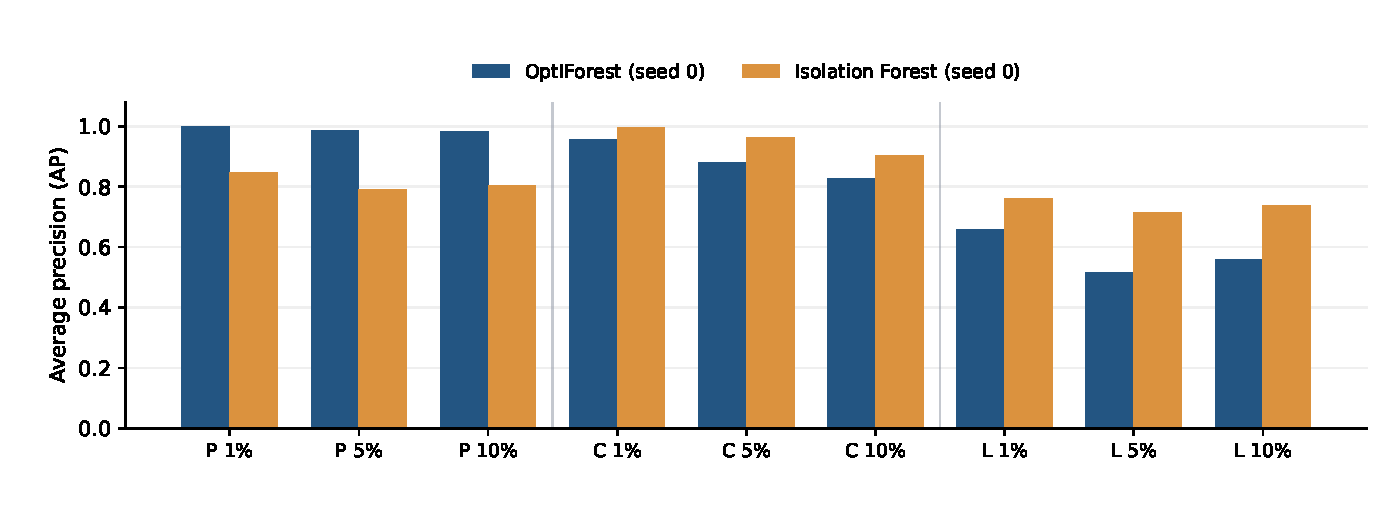
\includegraphics[draft=false,width=.91\textwidth]{figures/synthetic_ap.pdf}
\caption{Average precision for matched model seed 0 on each generated dataset. Labels P, C and L denote point, contextual and collective anomalies. The figure shows exploratory, not inferential, comparisons.}
\label{fig:synthetic}
\end{figure*}
 
In the three point-anomaly settings, OptIForest had higher seed-0 AP, with differences ranging from +0.1509 to +0.1944. In all contextual and collective settings, iForest had higher seed-0 AP. The largest observed disadvantage for OptIForest was collective 5\% ($\Delta\ap=-0.1980$). These results are compatible with the idea that detectability depends on how deviations are constructed; however, the injected mechanisms also modify marginal feature distributions, so the three families cannot be interpreted as a pure mechanism-isolation causal test. The contextual and collective results challenge a universal interpretation of H3.
 
\subsection{Repeated-run observations and cost}
The iForest baseline was run 15 times for each synthetic dataset. Its mean AP at 1\%, 5\%, 10\% prevalence was, respectively, 0.8144, 0.7727, 0.7461 for point anomalies; 0.9941, 0.9119, 0.8433 for contextual anomalies; and 0.8341, 0.7379, 0.7185 for collective anomalies. These values should not be silently compared with a single OptIForest replicate as if they had matching uncertainty.
 
Two OptIForest settings were also run on model seeds 0--2. Point 1\% obtained mean AP $0.9956$ (sample SD 0.0018), and point 5\% obtained mean AP $0.9907$ (sample SD approximately 0.0066). On the same model seeds, both exceed their matched iForest means. For the remaining seven datasets, only one OptIForest model seed was retained; a paired confidence interval for H3 across all settings is therefore unavailable. AP is influenced by positive-class prevalence, and separate generated datasets also differ in their normal/anomaly mixtures. Changes across prevalence are descriptive, not identified prevalence-only effects.
 
A clear performance--cost trade-off emerged. On synthetic point 1\%, OptIForest required about 9.66 seconds for fitting and 143.05 seconds for scoring one 10,000-row dataset; iForest's 15-seed mean fitting and scoring times were about 0.148 and 0.049 seconds. OptIForest scoring, not merely fitting, is the major cost under this implementation. Hardware, library versions and execution settings limit cross-system runtime generalisation.
 
 
\subsection{A narrow paired uncertainty analysis}
For the two point-anomaly datasets with three OptIForest model seeds, we can compare AP differences with iForest on the identical dataset and model seed. Defining $d_i=\ap_{\mathrm{Opt},i}-\ap_{\mathrm{iF},i}$, the sample mean $\bar d$ represents the observed effect, and a classical $t$ interval is $\bar d\pm t_{0.975,n-1}s_d/\sqrt{n}$. With only $n=3$, its assumptions and interval width require extreme caution. For point 1\%, the mean paired AP difference is $+0.1646$ and the approximate 95\% interval is $[-0.0117,0.3409]$. For point 5\%, the corresponding mean is $+0.2070$ with interval $[0.1464,0.2677]$. Although the latter interval is positive, both intervals capture only \emph{model randomness on a single generated dataset}; they are not confidence intervals over independent transaction populations or generator seeds.
 
\begin{table}[t]
\centering\small
\caption{Limited paired AP analysis on the two point datasets with three model seeds. Confidence limits are $t$ intervals with 2 degrees of freedom and should be read cautiously.}
\label{tab:paired}
\begin{tabular}{@{}lrrr@{}}
\toprule
Rate & Mean $\Delta$AP & Lower 95\% & Upper 95\% \\
\midrule
1\% & +0.1646 & $-0.0117$ & +0.3409 \\
5\% & +0.2070 & +0.1464 & +0.2677 \\
\bottomrule
\end{tabular}
\end{table}
 
This analysis illustrates why a large observed score gap should not immediately be called statistically significant. For point 1\%, the wide interval even includes a small negative difference, despite all three recorded differences being positive. There are only three possible seed pairings in the preserved OptIForest subset; adding many iForest-only seeds cannot compensate for missing OptIForest seeds. Prevalence-level comparisons also require care because the positive class's base rate changes the expected average precision of a random ranking (approximately the prevalence itself). Our reported AP values are therefore accompanied by ROC-AUC and always contextualised with the anomaly rate.
 
\section{Ethics and Data Management}
Responsible computational research requires accurate provenance, disclosure of limitations, transparent reporting and reproducibility, consistent with the Australian Code for the Responsible Conduct of Research \citep{nhmrc2018}. No personal financial or medical data were collected in the synthetic extension. Generated feature names imitate payment-system concepts but do not imply bank-grade realism, actual identities or consent from real users. The AD benchmark and upstream code require source attribution and careful review of their distribution conditions before public redistribution.
 
For a real financial screening deployment, false positives can block legitimate transactions and disproportionately burden particular customer groups; false negatives may fail to identify harmful behaviour. The present experiments do not assess subgroup fairness, individual impact, calibration or prospective monitoring. High discrimination metrics on injected synthetic anomalies cannot support claims of production fraud-detection effectiveness. Aggregate AP and ROC-AUC hide threshold-specific downstream workloads and operational costs.
 
The project also has research-integrity obligations: preserve original code provenance, identify the NumPy compatibility correction, store immutable CSV outputs and seeds, and document interrupted or incomplete runs. Threshold 7 has no completed numerical result; the warning in the tree implementation remains an unresolved numerical concern. Likewise, an exploratory finding should not be presented as statistically significant without repeated independent trials and uncertainty analysis. Releasing the generator and non-sensitive synthetic CSVs supports auditability, while credentials, identifiable data and unlicensed third-party datasets must not be committed to a public repository.
 
\section{Discussion and Conclusions}
RQ1 was addressed successfully for the accessible AD experiment: the mean ROC-AUC and AP closely reproduce the original reported figures. RQ2 revealed sensitivity to branch and threshold choice: ternary branching led the three-seed mean AP at threshold 403, whereas the highest single-seed AP and lowest runtime among tested cut thresholds occurred at 512. The threshold-7 computation was attempted but not completed; low thresholds can have prohibitive computational costs. Neither ablation supports universal parameter claims.
 
RQ3 yielded mixed evidence. OptIForest achieved very high AP on point anomalies for all three prevalences, with repeatability checks on point 1\% and 5\%. However, iForest had higher matched-seed AP on contextual and collective data. These outcomes argue against the assumption that a favourable original benchmark automatically translates across distinct anomaly-generation scenarios. The result is scientifically useful even though the initial superiority hypothesis is not broadly supported.
 
Key limitations include only one accessible original benchmark, generator seed 42 for synthetic files, mostly single-seed OptIForest measurements beyond point anomalies, limited ablation repetitions, lack of a validated real transaction dataset, and a transductive evaluation protocol. The collective generator does not record genuine relational groups; true collective anomaly research would require explicit sequences, entities or linked event annotations. Future studies should add more generator seeds, matched repeated model seeds, bootstrap or paired interval estimates, external benchmarks, and prospective holdout evaluation. We also recommend profiling the scoring implementation and auditing the recurring numerical warning before relying on runtime or robustness claims.
 
Overall, the project demonstrates a close partial reproduction of the published OptIForest result, transparent controlled experiments and reproducibly generated new datasets. Its strongest contribution is an evidence-based account of where the supplied implementation appears effective, where a simpler baseline compares favourably, and what remains uncertain.
 
 
\subsection{Threats to internal and external validity}
Several issues affect how confidently the observed differences can be attributed to the methods. First, numerical compatibility changes and the recurring invalid-division warning mean the precise behaviour of the upstream implementation deserves further inspection. We did not change the algorithm to silence the warning, avoiding an unvalidated modification, but this also means it remains unresolved. Second, no held-out validation set was used to select branch or threshold configurations; results at the available settings are exploratory and potentially subject to selection bias if one retrospectively chooses the best configuration. The default threshold 403, not the empirically best threshold 512, was retained for synthetic experiments to preserve a coherent baseline.
 
Third, model randomness was replicated more extensively for iForest than for OptIForest. Reporting matched single-seed results avoids one misleading comparison but does not remove the statistical limitation. Fourth, dataset-generation seed 42 was fixed for every reported prevalence--mechanism configuration, so changes attributed informally to prevalence could also reflect the newly drawn normal profiles or injected records. A more controlled prevalence analysis would hold normal records fixed and vary only anomaly injection, then replicate independently generated worlds. Fifth, the synthetic feature schema is small and constructed from assumptions rather than observed transactional dependencies. The strikingly high point anomaly scores, in particular, may largely measure sensitivity to exaggerated amount and velocity signals rather than complex fraud patterns.
 
Finally, total scoring time is method- and implementation-specific. Unlike throughput benchmarks on production infrastructure, these experiments ran locally, with no detailed control for hardware thermals, thread scheduling, process contention or caching. Runtime differences are large enough to motivate further profiling, but statements about production latency would require measured throughput and deployment-relevant resource controls. Taken together, these threats limit generalisation while leaving the transparent code-replication exercise informative.
 
\section{Reproduction Checklist and Artifact Scope}
The supplied project archive distinguishes three forms of research evidence: source code (the upstream implementation and locally written wrappers), generated data (nine CSVs with corresponding JSON sidecars), and saved model results (seed-indexed CSVs). Each record in the baseline CSV contains its model seed, ROC-AUC, AP, fitting time and scoring time. The ablation files additionally identify the tree count, branch and threshold. A result with one row corresponds to a single stochastic model run, even when the matching baseline file includes fifteen rows. This is why the single-seed comparison and repeated-baseline summaries are presented separately.
 
The audit procedure is straightforward. First, verify the dataset shape and metadata checksums and confirm that no label column enters fitting. Second, inspect the exact OptIForest model configuration and record both Python and NumPy random seeds. Third, recalculate AP and ROC-AUC from the same score orientation; OptIForest scores were inverted in the local wrapper because lower native scores indicate greater anomaly. Fourth, compare each reported table against the saved seed-indexed CSVs. Fifth, preserve all failed or interrupted attempts without assigning them an accuracy value. In particular, the threshold-7 run should never appear as a missing zero or be included in a numerical average.
 
For an independent replication, the GitHub repository should be cloned into a fresh environment, the pinned dependencies installed, and \texttt{demo.py} and the experiment wrappers invoked with documented commands. If the original source is kept as a third-party subfolder, the README must identify that origin rather than present it as the student's own algorithm. The local source patch should be kept minimal and reviewable. Publishing CSV outputs is not a substitute for making the experiment runnable, but it allows a grader to inspect computations without rerunning the most expensive low-threshold configurations.
 
\section*{Code and Reproducibility Statement}
Scripts, synthetic data, metadata and CSV results are supplied in the companion archive. The report must link to a \emph{publicly accessible} GitHub repository before submission: \repository. The GitHub README should document the Python environment, source-code attribution, original-data execution and synthetic experiment commands. Repository availability and a working link have not yet been verified and must not be claimed until publishing is complete.
 
\IfFileExists{acl_natbib.bst}{\bibliographystyle{acl_natbib}}{\bibliographystyle{plainnat}}
\bibliography{custom}
\end{document}
